\begin{figure}[!h]
    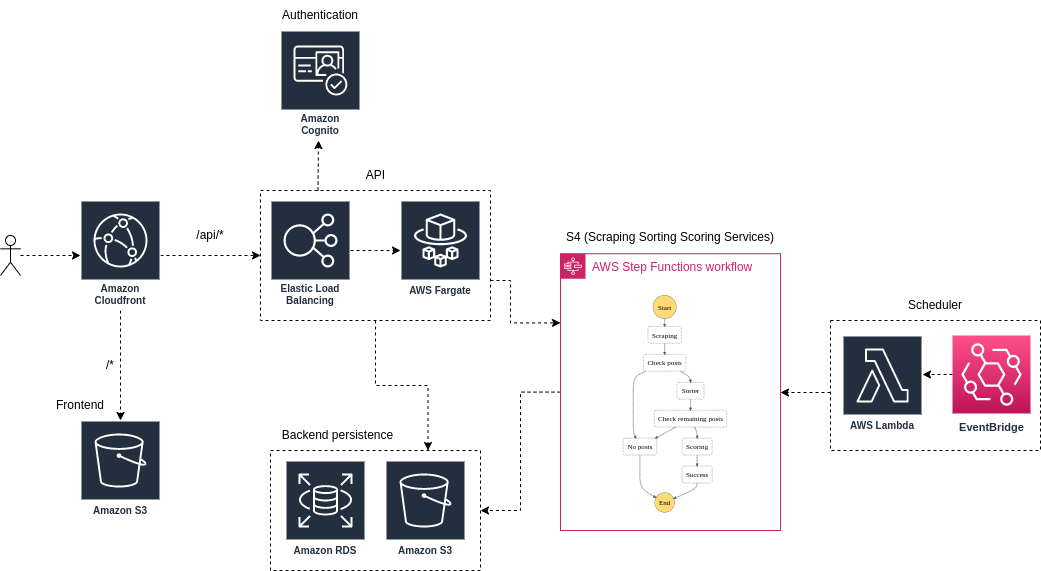
\includegraphics[width=16cm]{sezioni/images/overview.png}
    \centering
    \caption{Visione d'insieme del sistema}
\end{figure}

\subsection{Descrizione generale}
Il Backend\G{} della piattaforma sfrutta un'architettura a microservizi, i quali comunicano fra di loro secondo regole e meccanismi appropriati.
Le varie parti sono fra di loro indipendenti e i dati da esse prodotti persistono in Amazon RDS\G{} o bucket\G{} S3, a seconda della lora natura.
Il lavoro di analisi e progettazione ha permesso di individuare i seguenti servizi:
\begin{itemize}
    \item \textbf{API Service}: ha il compito di far interfacciare il Frontend\G{} con il resto del sistema, in particolare fornisce
    delle API\G{} RESTful che consentono l'ottenimento dei dati dal database e in generale di gestire tutte le funzionalità rese disponibili all'utente;
    \item \textbf{Signup Service}: risponde agli eventi \textit{pre signup} di Amazon Cognito\G{} e permette di aggiungere automaticamente utenti al database della piattaforma, dopo la loro registrazione;
    \item \textbf{S4} (\textbf{S}craping \textbf{S}orting \textbf{S}coring \textbf{S}ervices):
        \begin{itemize}
            \item \textbf{Scraping Service}: sfruttando apposite tecniche e librerie, effettua operazioni di scraping\G{} da Instagram\G{} al fine di ottenere dati che
            saranno successivamente processati dagli altri servizi;
            \item \textbf{Sorting Service}: effettua un preprocessing sui dati ottenuti dallo scraping\G, scartando eventuali dati non conformi e che comporterebbero
            uno spreco di risorse nelle fasi successive di analisi;
            \item \textbf{Scoring Service}: esegue analisi approfondite su dati testuali e multimediali, producendo una valutazione numerica; 
        \end{itemize}
    \item \textbf{Scheduler Service}: programma l'esecuzione di \textbf{S4} secondo un intervallo di tempo predefinito.
\end{itemize}

\subsection{Servizi S4}
I servizi di scraping, sorting e scoring formano un raggruppamento logico chiamato \textbf{S4} (\textbf{S}craping \textbf{S}orting \textbf{S}coring \textbf{S}ervices).
Essi vengono eseguiti in funzioni Lambda, le quali sono orchestrate attraverso \textit{AWS Step Functions}.
\begin{figure}[H]
    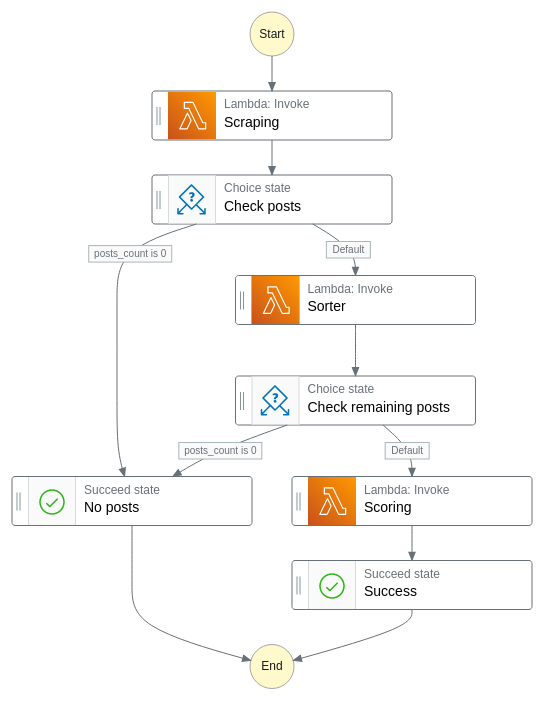
\includegraphics[width=8cm]{sezioni/images/stepfunctions_graph.png}
    \centering
    \caption{Visualizzazione macchina a stati}
\end{figure}
L'orchestratore permette di definire il flusso di esecuzione come una macchina a stati, dove l'output di uno stato
diventa l'input di quello successivo.\\
Uno stato può anche controllare il flusso dell'esecuzione, per esempio se dopo
l'operazione di sorting non restano post da analizzare e quindi da passare in input al servizio di scoring, si arriva
subito ad uno stato terminale che quindi termina l'esecuzione senza sprecare risorse.

\newpage

\subsection{Database}
La persistenza dei dati è affidata ad un database relazionale, su DBMS\G{} \textit{PostgreSQL}.
Il database è gestito dal servizio \textit{Amazon RDS}\G.
\begin{figure}[H]
    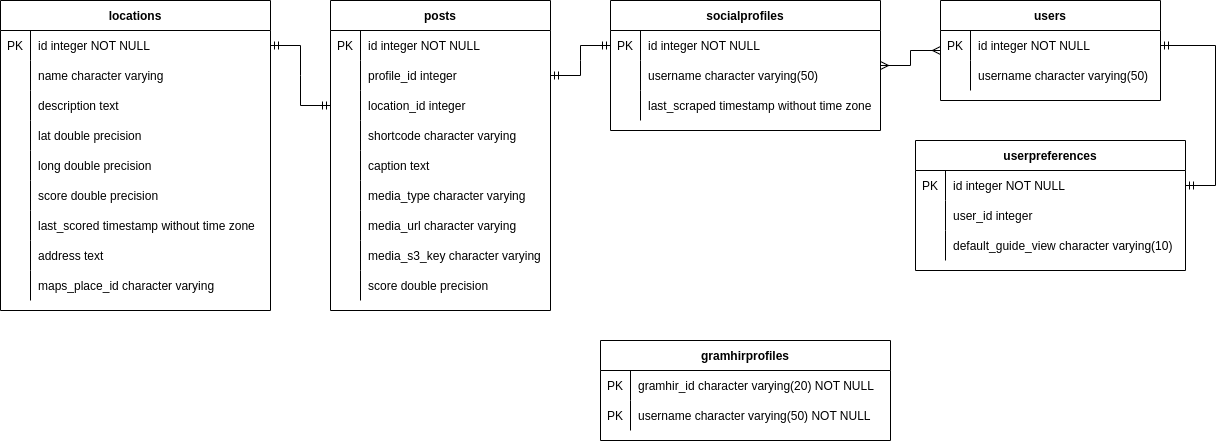
\includegraphics[width=15cm]{sezioni/images/db_er.png}
    \centering
    \caption{Schema ER database}
\end{figure}

\subsubsection{Interfacciamento}
L'interfacciamento con il database, da parte dei vari servizi, è affidato alla libreria Python\G{} \textit{SQLAlchemy}.
Essendo una libreria ORM\G{}, vengono definiti dei modelli che permettono l'interazione con le entità e le relazioni
interne al database come dei normali oggetti.

\subsubsection{Versionamento}
Il versionamento della schemo relazione del database è affidato allo strumento \textit{alembic}, che in
sintonia con la libreria sopracitata \textit{SQLAlchemy}, gestisce in automatico i cambiamenti apportati allo schema.
Questi cambiamenti vengono raggruppati in operazioni atomiche dette migrazioni.

\begin{lstlisting}[language=Python, caption=Esempio di migrazione autogenerata]
"""add location address and maps_place_id
Revision ID: 6ce8d444b850
Revises: a557f1403100
Create Date: 2022-09-01 10:43:05.074767
"""

from alembic import op
import sqlalchemy as sa

# revision identifiers, used by Alembic.
revision = '6ce8d444b850'
down_revision = 'a557f1403100'
branch_labels = None
depends_on = None

def upgrade() -> None:
    # ### commands auto generated by Alembic - please adjust! ###
    op.add_column('locations', sa.Column('address', sa.Text(), nullable=True))
    op.add_column('locations', sa.Column('maps_place_id', sa.String(), nullable=True))
    # ### end Alembic commands ###

def downgrade() -> None:
    # ### commands auto generated by Alembic - please adjust! ###
    op.drop_column('locations', 'maps_place_id')
    op.drop_column('locations', 'address')
    # ### end Alembic commands ###
\end{lstlisting}
